\documentclass[12pt,a4paper]{article}
\usepackage{graphicx}
\usepackage{polski}
\usepackage[utf8]{inputenc}
\title{Sprawozdanie z laboratorium PAMSI}
\author{Damian Oleksak}
\date{}
\begin{document}
\maketitle

Sortowanie heapsort polega na wykorzystaniu kopca binarnego. Na początku budowany jest z wszystkich elementów kopiec, którego korzeń jest elementem największym. Następnie kolejne największe elementy są wstawiane na odpowiednie miejsca w tablicy, natomiast elementy zajmujące te miejsca są wstawiane na szczyt kopca i jest on odbudowywany w dół za pomocą operacji Heapify.

Algorytm budowy kopca działa w ten sposób, że buduje najpierw małe kopce, z elementów znajdujących się na końcu tablicy, i później - idąc "w górę" tablicy - kopce te łączone są w większe, aż do powstania całego kopca. Ponieważ elementy znajdujące się w "dolnej" połówce tablicy są liśćmi kopca - nie trzeba z nich budować małych kopców (same są kopcami jednoelementowymi). 

Algorytm sortowania przez kopcowanie zalicza się do algorytmów szybkich. Jego złożoność jest liniowo-logarytmiczna - O(n*log(n)). Jest około 3 razy wolniejszy od sortowania szybkiego.\newline


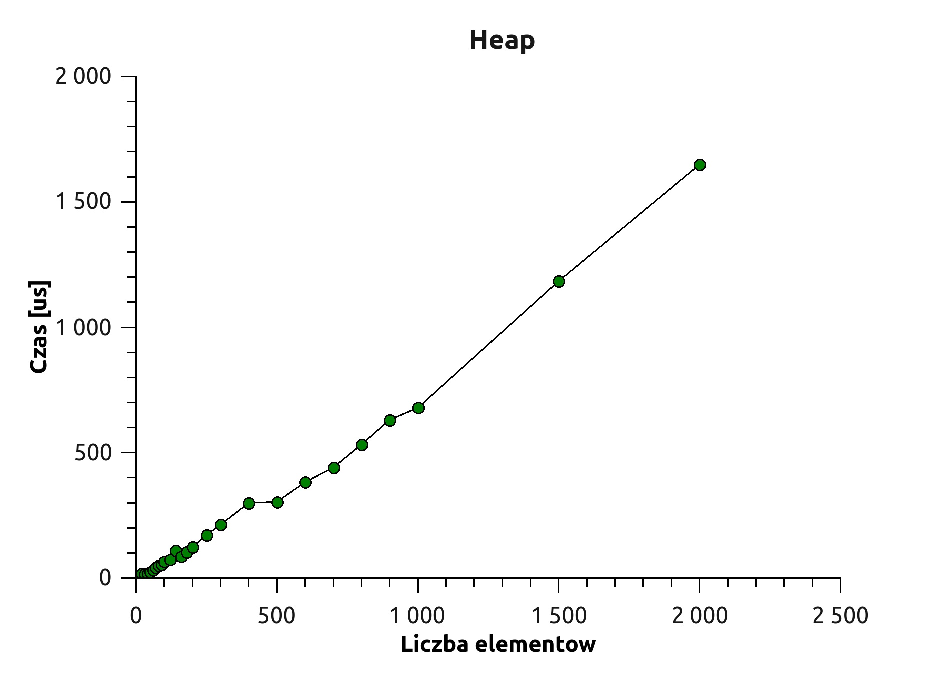
\includegraphics[scale=0.8]{./heap}

Wykres 1. Sortowanie przez kopcowanie \newpage

Sortowanie szybkie (quicksort) jest używane w sytuacjach, gdy sortuje się duże ilości
danych – gdy danych jest niewiele, proste algorytmy sortowania są efektywniejsze. Jako granicę
sensowności stosowania sortowania algorytmem quicksort przyjmuje się zwykle ilość sortowanych
elementów, wynoszącą minimum 10. Złożoność obliczeniowa jest rzędu O(n*log(n)), lecz w przypadku pesymistycznym O($n^{2}$) - sortowanie przez kopcowanie okazuje się szybsze.\newline

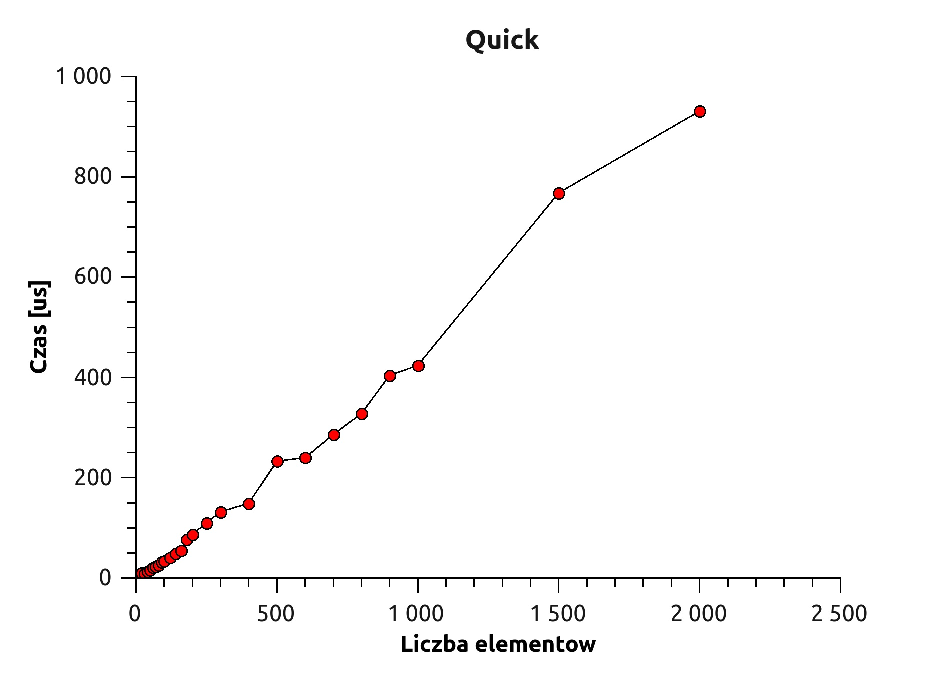
\includegraphics[scale=0.8]{./quick}

Wykres 2. Sortowanie szybkie \newpage

Sortowanie przez scalanie, podobnie jak algorytm quicksort, jest algorytmem typu "dziel i zwyciężaj". Jednak w odróżnieniu od sortowania szybkiego, algorytm ten w każdym przypadku osiąga złozoność O(n*log(n)). Niestety algorytm mergesort posiada większą złożoność pamięciową, potrzebuje do swojego działania dodatkowej, pomocniczej struktury danych.
Ideą działania algorytmu jest dzielenie zbioru danych na mniejsze zbiory, aż do uzyskania n zbiorów jednoelementowych. Następnie zbiory te są łączone w coraz większe zbiory posortowane, aż do uzyskania jednego, posortowanego zbioru n-elementowego.\newline

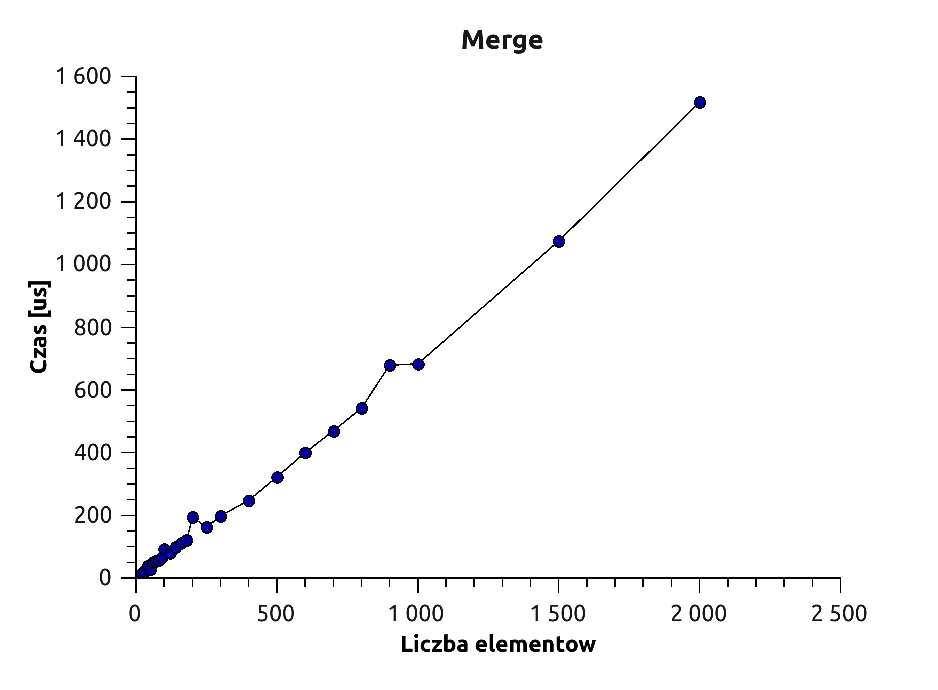
\includegraphics[scale=0.8]{./merge}

Wykres 3. Sortowanie przez scalanie \newpage

Wykresy zostały wygenerowane na podstawie pomiarów czasu sortowania losowo wygenerowanych elementów od ich liczby.    \newline

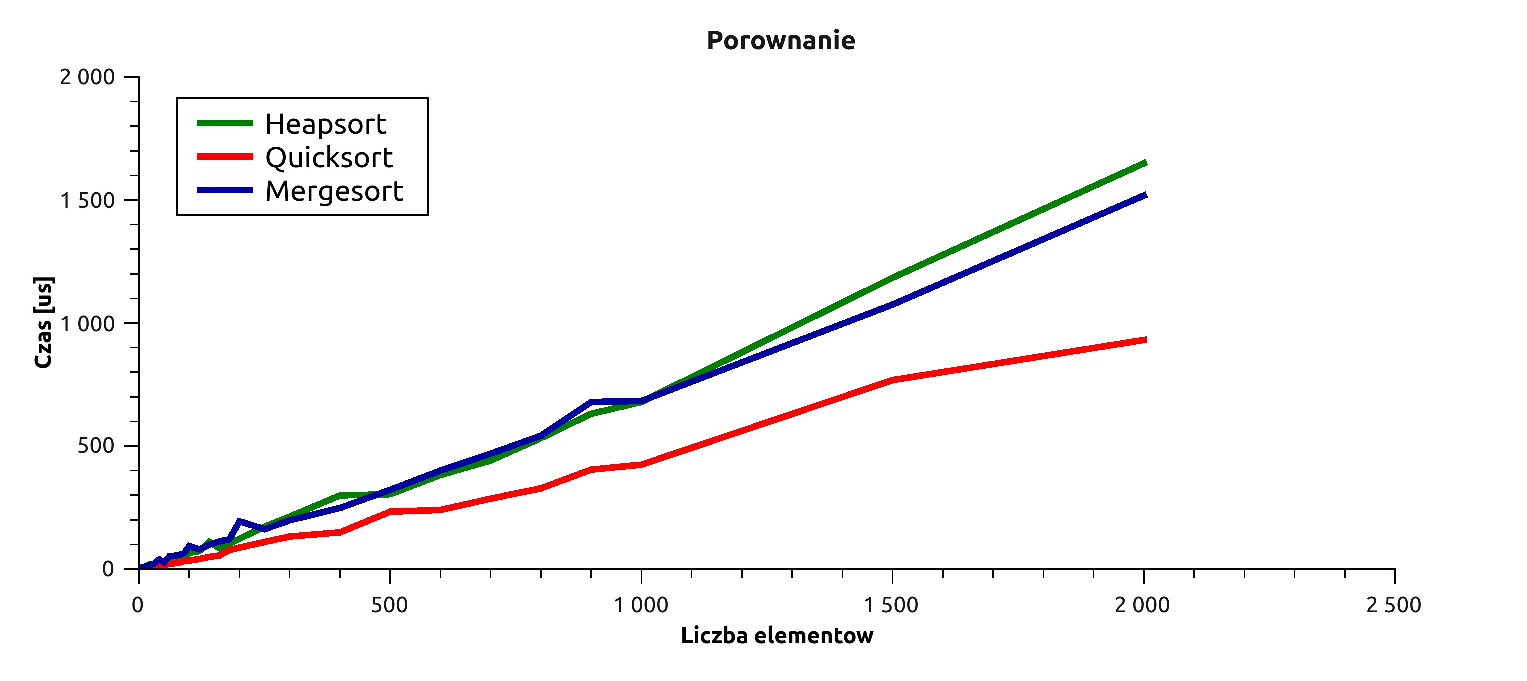
\includegraphics[scale=0.6]{./wszystkie}

Wykres 4. Porównanie wszystkich algorytmów sortowania \newline

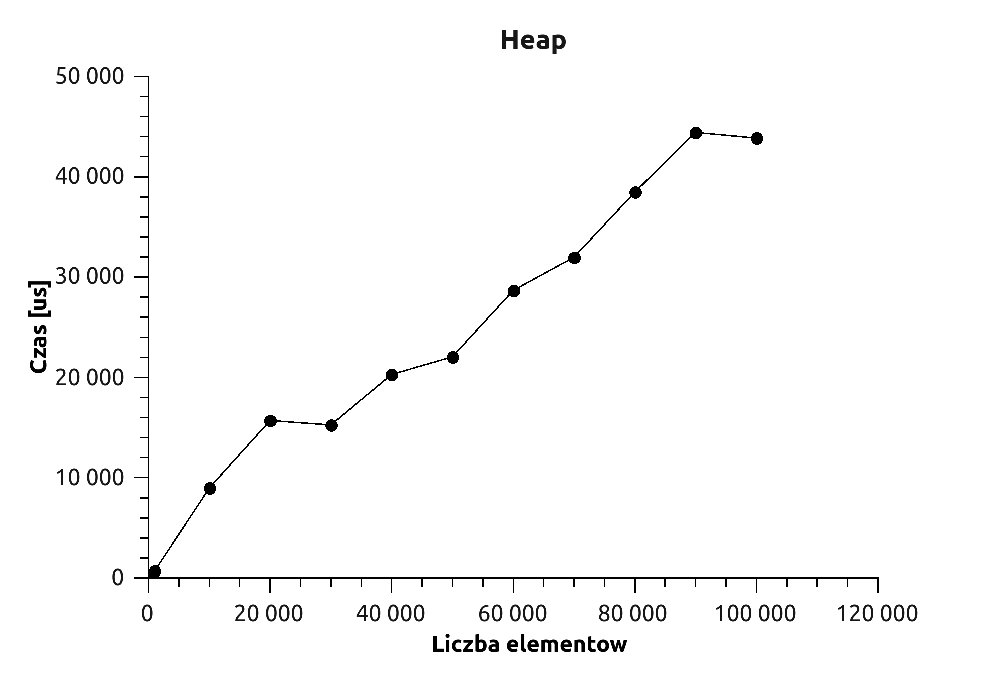
\includegraphics[scale=0.8]{./wiecejelem} \newline
Wykres 5. Wykres Heapsort dla wiekszej liczby elementow. \newline

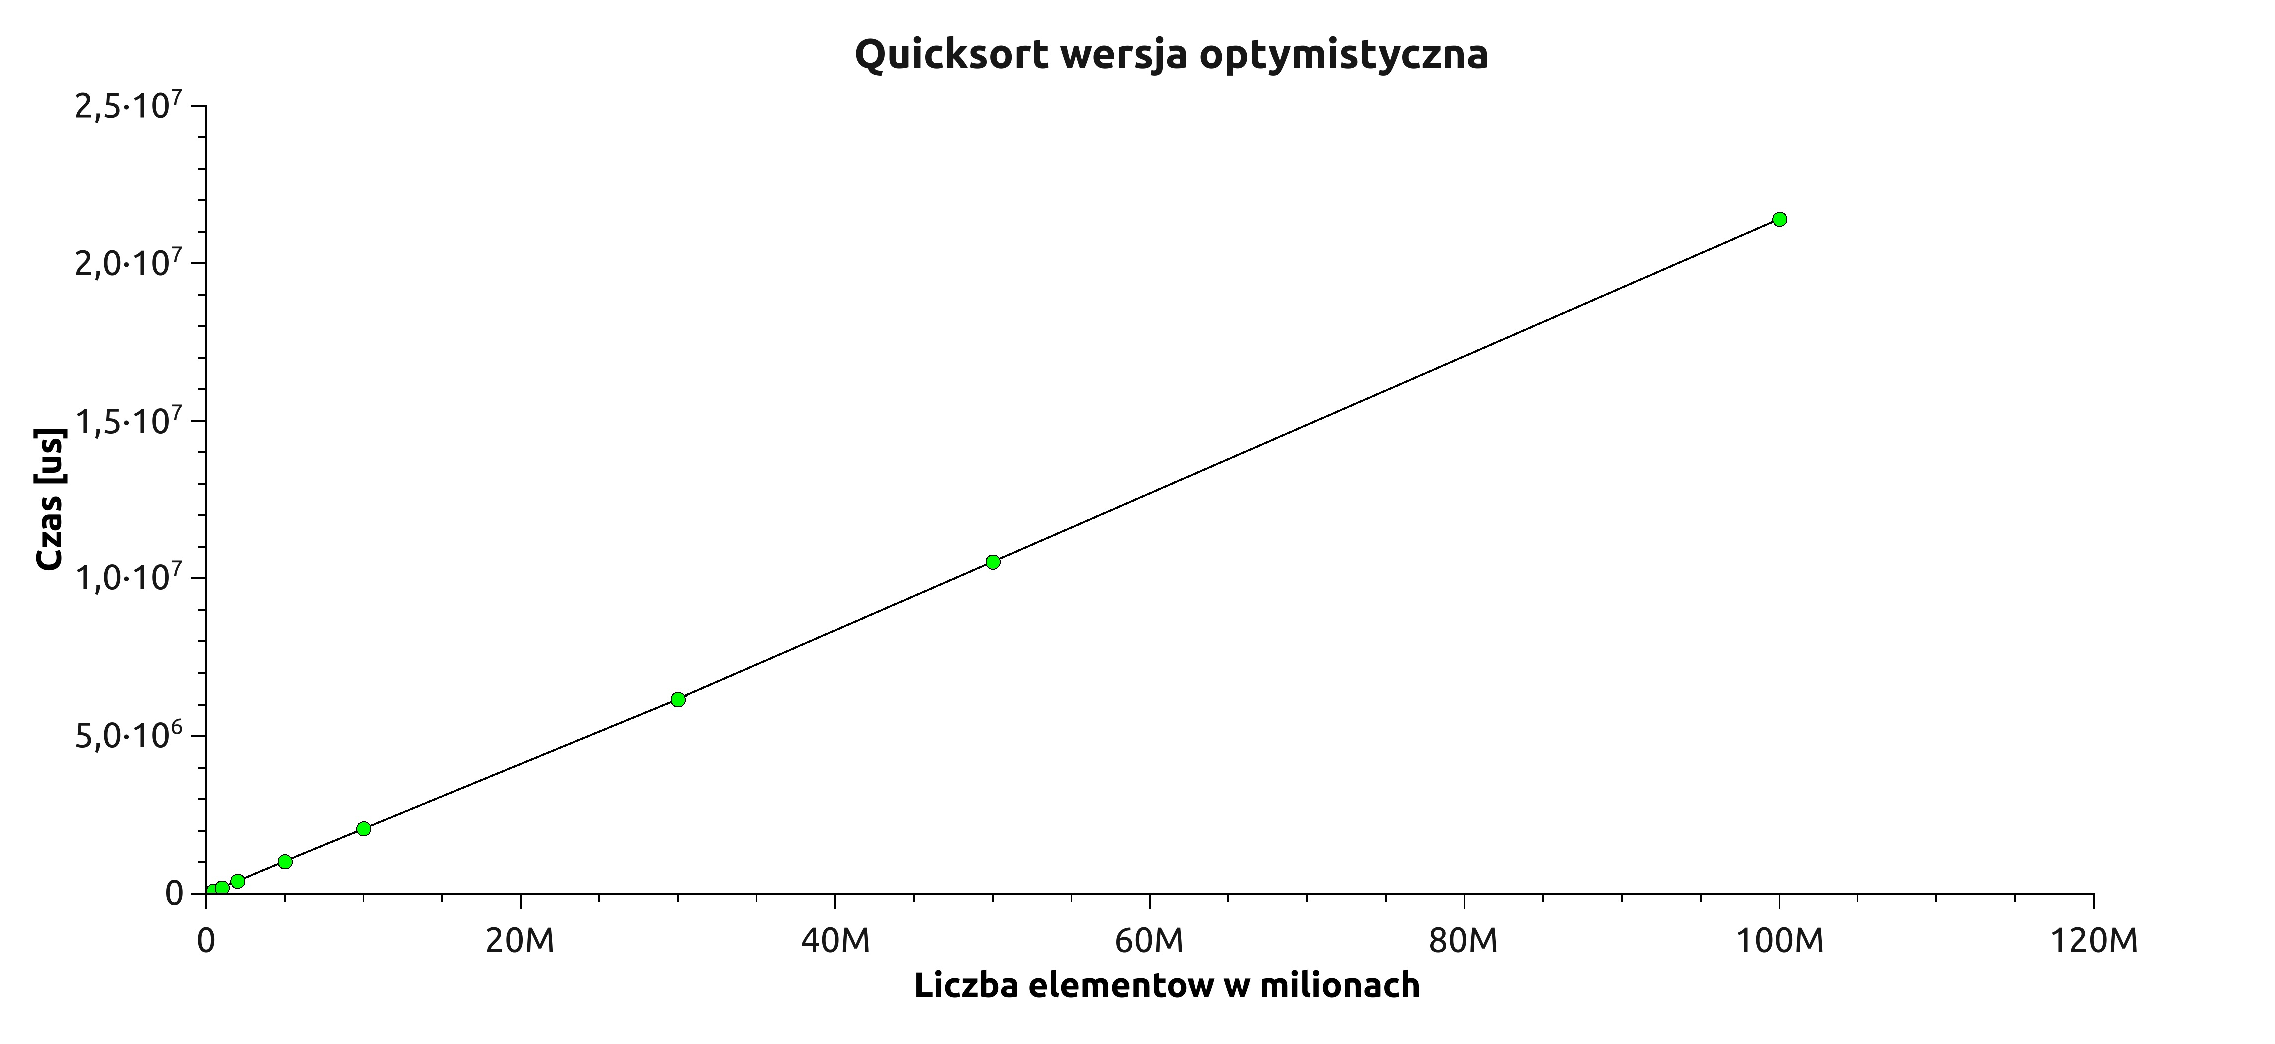
\includegraphics[scale=0.4]{./qopt} \newline
Wykres 6. Wykres Quicksort dla wariantu sortowania do 100 mln losowo generowanych elementów. Algorytm wybiera skrajny element tablicy do podziału. \newpage

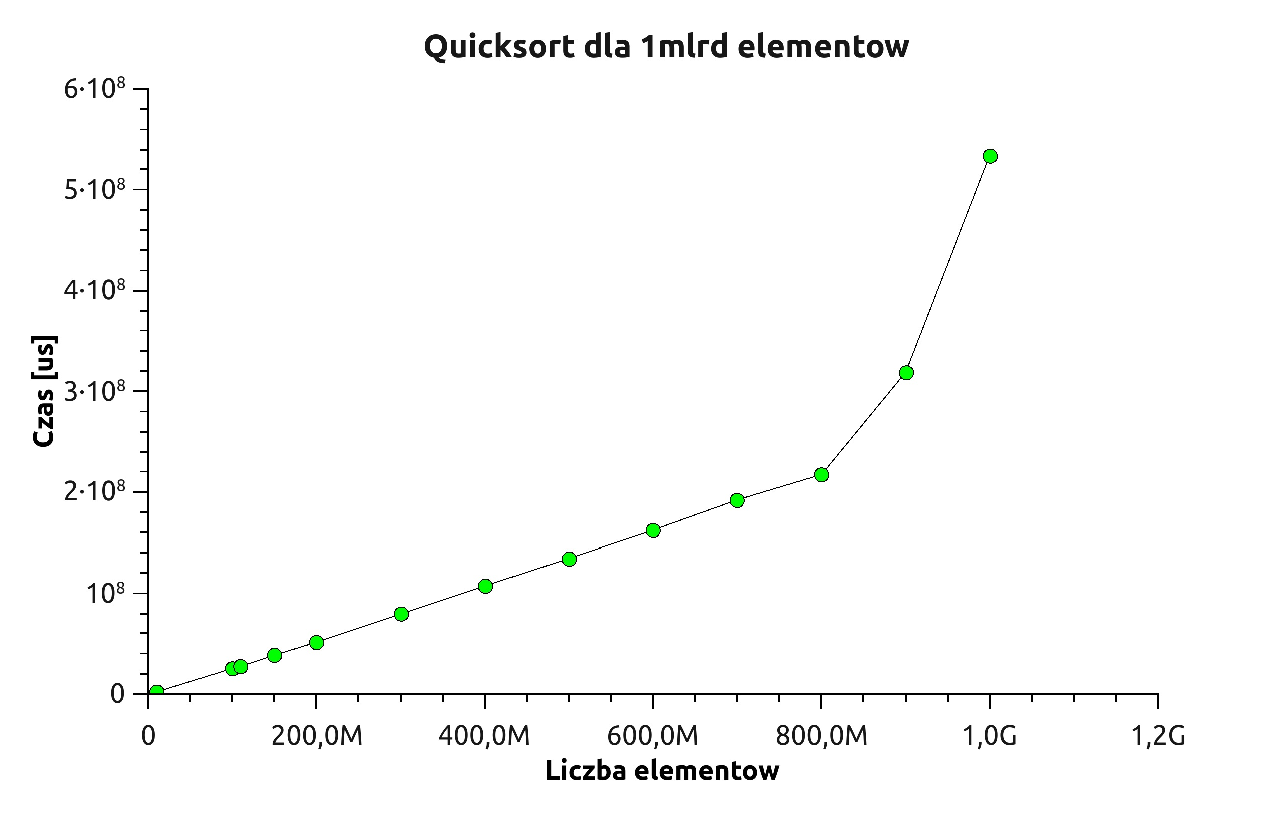
\includegraphics[scale=0.4]{./qmld} \newline
Wykres 7. Wykres Quicksort dla wariantu sortowania do miliarda losowo generowanych elementów. Algorytm wybiera skrajny element tablicy do podziału. Dopiero teraz widać wyraźne zagięcie
krzywej. \newpage

\includegraphics[scale=0.6]{./qpes} \newline
Wykres 8. Wykres Quicksort dla wariantu pesymistycznego- sortowanie do 100 tys już posortowanych elementów. Algorytm wybiera skrajny element tablicy do podziału. \newpage

\includegraphics[scale=0.6]{./qmal} \newline
Wykres 9. Wykres Quicksort dla wariantu pesymistycznego- sortowanie do 100 tys posortowanych elementów w kolejności malejącej. Algorytm wybiera skrajny element tablicy do podziału. \newpage

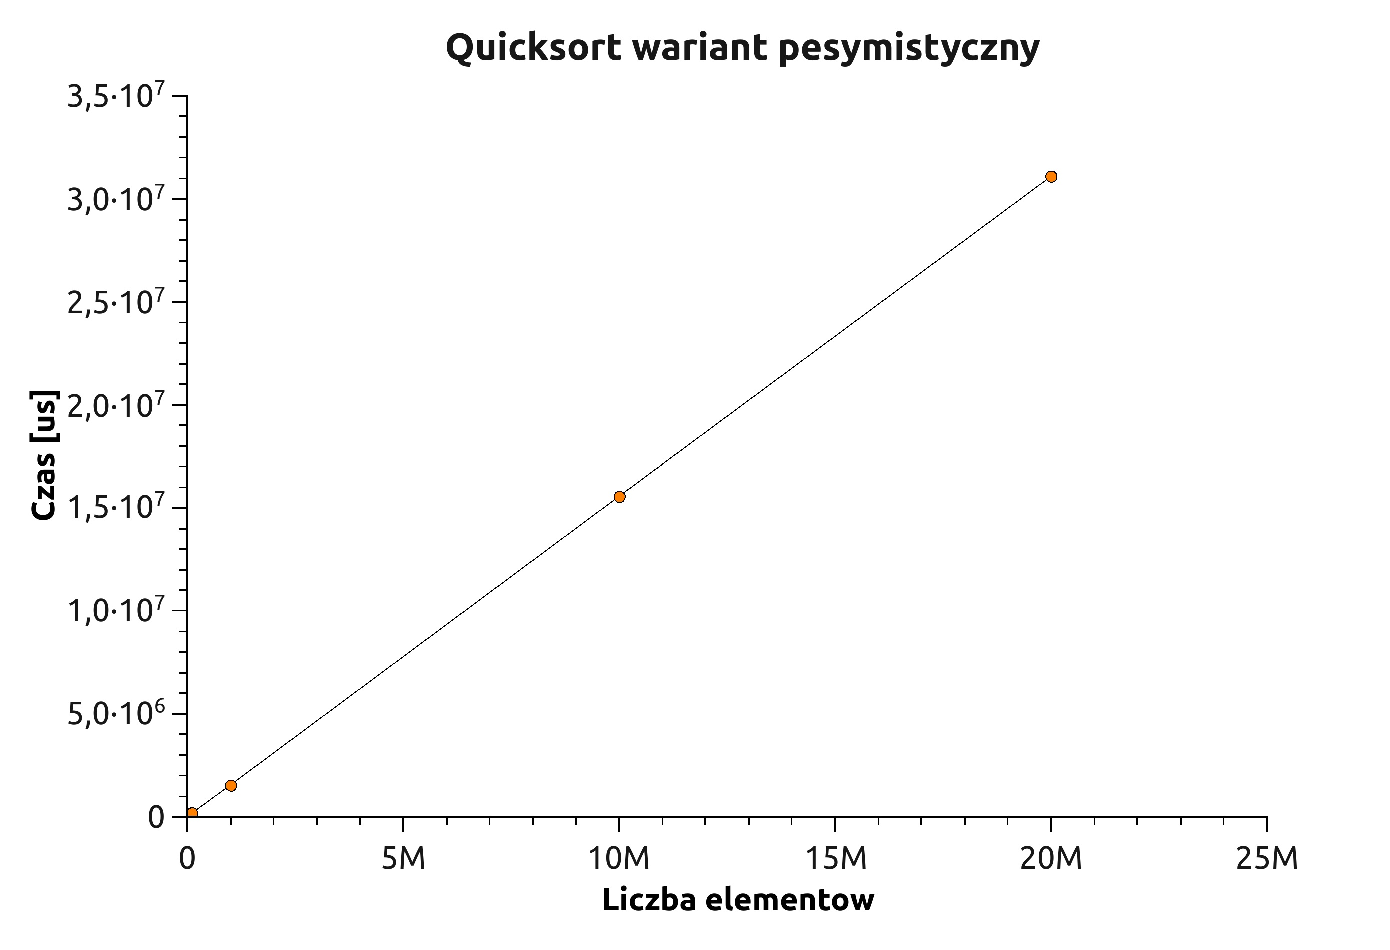
\includegraphics[scale=0.6]{./qpn} \newline
Wykres 10. Wykres Quicksort dla wariantu pesymistycznego- sortowanie do 20 mln już posortowanych elementów. Algorytm wybiera element do podziału poprzez losowanie. Pozwala to zniwelować prawdopodobieństwo wystąpienia kwadratowej złożoności obliczeniowej. Jednak dla przypadku, gdy dane wejściowe nie były posortowane, algorytm wybierania skrajnego elementu do podziału okazywał się szybszy.

\end{document} 
